\documentclass[12pt]{article}
\usepackage[utf8]{inputenc}
\usepackage[T2A]{fontenc}
\usepackage[russian]{babel}
\usepackage{amsmath}
\usepackage{amssymb}
\usepackage{dsfont}
\usepackage[dvipsnames]{xcolor}
\usepackage{setspace}
\usepackage{multirow}
\usepackage[a4paper, outer=1.5cm, inner=1.5cm, top=1cm, bottom=1cm]{geometry}
\usepackage{graphicx}
\usepackage{skull}
\usepackage{wasysym}
\usepackage{float}
\graphicspath{{.images/}}
\usepackage{hyperref}
\hypersetup{colorlinks=true, linkcolor=blue, filecolor=magenta, urlcolor=cyan}
\usepackage[firstpage]{draftwatermark}
\SetWatermarkText{
    $\qquad\qquad\qquad\qquad\qquad$\parbox{7cm}{\begin{center}
    
\includegraphics[width = 0.08\textwidth]{lion-logo.png}\bigskip\\~\bigskip\\~\vspace{-24mm}\\~\end{center}}
}
\SetWatermarkAngle{0}
\SetWatermarkScale{1.5}
\usepackage{etoolbox}

\newtoggle{ifsolved}
\newtoggle{needhelp}
\newcounter{num}
\setcounter{num}{1}

\newcommand{\newnum}{\par\textbf{\textnumero\arabic{num}}\stepcounter{num}}
\newcommand{\sol}{\vspace{3mm}\par\textbf{Решение: }}
\newcommand{\ans}{\vspace{3mm}\par\textbf{Ответ: }}
\newcommand{\hint}{\vspace{3mm}\par\textbf{Подсказка: }}
\newcommand{\mode}[1]{
\ifstrequal{#1}{0}{\togglefalse{ifsolved}\togglefalse{needhelp}}{\ifstrequal{#1}{1}{\togglefalse{ifsolved}\toggletrue{needhelp}}{\ifstrequal{#1}{2}{\toggletrue{ifsolved}\togglefalse{needhelp}}{\toggletrue{ifsolved}\toggletrue{needhelp}}}}} %if 0 - if 1 - if 2 - else
%\newenvironment{problem}[8]{%#1, #2, #3
%\parbox{\linewidth}{\vspace{4mm}\ifstrequal{#4}{(лёгкая)}{\newnum\textbf{.}}{\newnum\textbf{*.} } \\ #5}
%\iftoggle{ifsolved}{\sol #6}{}
%\iftoggle{ifsolved}{\ans #7}{}
%\iftoggle{needhelp}{\hint #8}{}}

\newenvironment{problem}[8]{%#1, #2, #3
\parbox{\linewidth}{\vspace{5mm}\ifstrequal{#4}{(лёгкая)}{\newnum\textbf{.}}{\newnum\textbf{*.} } \\ #5}
\iftoggle{ifsolved}{\sol #6}{}

\iftoggle{ifsolved}{\parbox{\linewidth}{\ans #7}}{}
\iftoggle{needhelp}{\parbox{\linewidth}{\hint #8}}{}}

\newenvironment{mylist} %custom list
{ \begin{itemize}
    \setlength{\itemsep}{0pt}
    \setlength{\parskip}{0pt}
    \setlength{\parsep}{0pt}     }
{ \end{itemize}                  }

\newenvironment{homeass}[1]{\vspace*{-1.5cm}
\iftoggle{ifsolved}{
    \section*{\center{Решение домашнего задания к #1.}}
}{
    \section*{\center{\textcolor{Sepia}{Домашнее задание к #1}}}
} \vspace{7mm}\large}

\parindent=0pt
\pagestyle{empty}
%$\!$[\arabic{class}.\arabic{num}]
%\ifnumcomp{\value{counter}}{>}{1}{true}{false}
%\definecolor{Gray}{gray}{0.9}
%\definecolor{mypink}{RGB}{219, 48, 122}
%\newcolumntype{g}{>{\columncolor{Gray}}p{2.8cm}}

\begin{document}
\large
\mode{7}
%0 for problems without hints
%1 for problems + hints
%2 for problems + solutions + answers
%else: show all

{\centering\section*{СПИСОК ЗАДАЧ}}

{\centering\subsection*{\smallskip\\\textcolor{green}{\textbf{Полезные вещи, которые можно и нужно копипастить:}}}}

\subsection*{\textcolor{Emerald}{\textbf{Полезные шпаргалки по LaTeXу:}}}

\textbf{Пример вставки рисунка:}

\begin{minipage}{\linewidth}
    \begin{minipage}{0.54\linewidth}
    см. рисунок справа\\
    Текст к собственно пикче, примерно всегда это либо развёрнутое описание, либо большая часть решения задачи --- стремимся экономить пространство, если это можно сделать.
    \end{minipage}
    \hspace{0.05\linewidth}
    \begin{minipage}{0.4\linewidth}
    \begin{figure}[H] 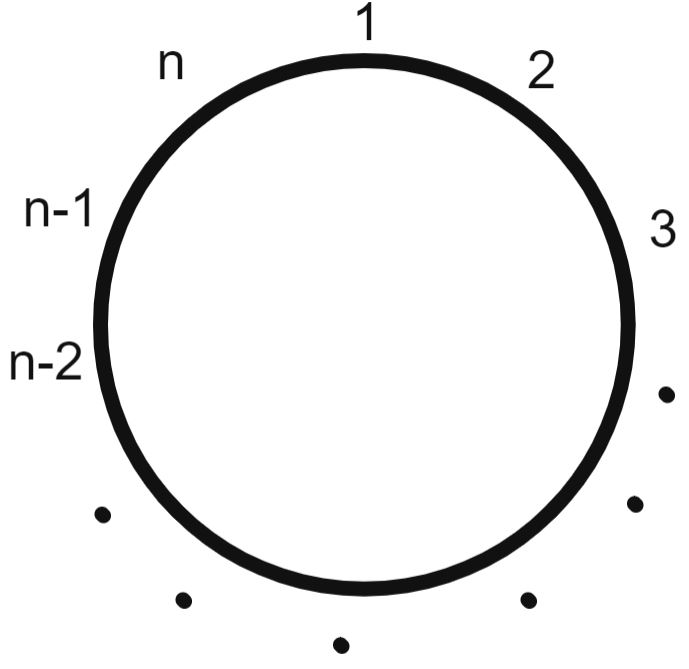
\includegraphics[width=\linewidth]{sol3} %тут поменять имя пикчи
    \end{figure}
    \end{minipage}
\end{minipage}

\textbf{Дефолтные математические знаки и символы:}\\
$\geqslant$,
$\leqslant$,
$a^{b}$,
$x_{i}$,
$\sqrt{a}$,
$\frac{a}{b}$,
$\displaystyle \frac{a}{b}$,
$\cdot$
$\;\Rightarrow\;$,
$\;\Leftrightarrow\;$,
$1{,}2$.
О промежутках:
$a\!b$,
$a\,b$,
$a\:b$,
$a\;b$,
$a\quad b$.

\textbf{Стандартные система и совокупность уравнений / неравенств:}\\
$\left\{
\begin{aligned}
f(x) &= 0 \\
g(x) &= 1
\end{aligned}\right.$

$\left[\begin{aligned}
&\left\{\begin{aligned}
f(x) &\geqslant a \\
g(x) &= b
\end{aligned}\right.\\
&\left\{\begin{aligned}
f(x) &< a \\
g(x) &= -b
\end{aligned}\right.
\end{aligned}\right.$

\subsection*{\textcolor{Emerald}{\textbf{Не математическое, но полезное:}}}
% комментарий в любом месте документа, который нигде не будет видно. Можно использовать для написания заметок-вопросов по задачам
\textbf{Пример таблицы:}

\begin{tabular}{|c|c|c|}
\hline
    $a$ & $b$ & текст
\\\hline
    $c$ & $d$ & мораль
\\\hline
\end{tabular}\\

\textbf{Отступы:} между\smallskip\\ строками\medskip\\ \textbf{Тире} --- это три дефиса.\\
\textbf{Списки:}
\begin{mylist}
\item [$\bullet$] это был пункт а
\item [2)] а это уже пункт номер 2 с изменённым заголовком
\end{mylist}

\subsection*{\textcolor{Emerald}{\textbf{Всё, неупомянутое выше (или если просто что-то не так):}}}
\begin{mylist}
\item [$\bullet$] Решение отдельных вопросов касательно ТеХа нужно искать в \href{https://www.mccme.ru/free-books/llang/newllang.pdf}{Львовском}.

\item [$\bullet$] Найти произвольный символ, который нужен, можно в \href{http://detexify.kirelabs.org/classify.html}{Detexify}.

\item [$\bullet$] Если возникли сомнения при решении, ответ практически ко всем задачам можно проверить с помощью \href{https://www.wolframalpha.com/}{WolframAlpha}.

\item [$\bullet$] Если в задаче нужно создать картинку, то лучше пока отложить эту задачу. Все графики планируется централизованно нарисовать (или перерисовать) в геогебре.

\item [\textcolor{brown}{\textbf{!!}}] Важно ставить \textcolor{red}{\textbf{$\spadesuit$}}
(или просто red) в тело задачи в случае серьёзных вопросов к решению и какой-то вопиющей лажи.

\item [\textcolor{brown}{\textbf{!!}}] Важно ставить \textcolor{olive}{\textbf{$\spadesuit$}}
(или просто olive) в тело задачи в случае не самого удачного текста и кривых отступов.
\end{mylist}

\subsection*{\textcolor{Violet}{\textbf{Комментарии:}}}% а также невидимые комментарии - так можно оставлять заметки-вопросы прямо в задаче, чтобы потом было понятно, в чём вопрос.
\begin{mylist}
\item [$\skull$] Переставлять задачи местами --- очень плохая идея.

\item [$\smiley$] При двойном клике по тексту pdf справа происходит автоматический переход к этому месту в латех-коде, а для обратного перехода можно нажать стрелку вправо (висит сверху между pdf и латех-кодом).

\item [$\smiley$] Если есть размышления, дописывать red/olive к задаче или не дописывать, то лучше всё-таки дописать.

\item [$\skull$] Самое плохое, что можно сделать --- написать в любое поле из трёх (НаписанноеРешение/ВерныйОтвет/Подсказка) только половину того, что надо, никак это не отметить, и потом пойти дальше.\\ Нужно в этот момент писать red/olive в случайном месте задачи, чтобы потом вычислить это с помощью Ctrl+F по всему документу (и это то, что потом будет делаться долго и тщательно)
\end{mylist}

\newpage
\setcounter{num}{462}

\hypertarget{7.1}{{\centering\section*{\bigskip\\\textcolor{Blue}{\hyperlink{start2}{\textcolor{Blue}{7.1}} Введение в алгебру.}\vspace{-5mm}}}}

\begin{problem}{Числовые выражения.}{7.1.1}{6K}{(лёгкая)}
{Два самолёта вылетели одновременно из Москвы в одном и том же направлении: один~--- со скоростью $350$ км/ч, а другой~--- со скоростью $280$ км/ч.\\ Через два часа первый самолёт уменьшил скорость до $230$ км/ч.\\ На каком расстоянии от Москвы второй самолёт догонит первый?\\ Составить числовое выражение по задаче (для расстояния до Москвы).}
{За два часа первый самолёт пролетел $350 \cdot 2 = 700$ км, а второй~--- $280 \cdot 2 = 560$ км. Значит, расстояние между самолётами будет равно $700 - 560 = 140$ км. Когда первый самолёт уменьшает скорость до 230 км/ч, получается, что скорость сближения самолётов равна $280 - 230 = 50$ км/ч. Значит, на то, чтобы догнать первый самолёт, понадобится ещё $\frac{140}{50} = \frac{14}{5} = 2{,}8$ часа $=$ 2 часа 48 мин. Второй самолёт за это время пролетит $280 \cdot 2{,}8 = 28\cdot28 = 784$ км. Следовательно, расстояние до Москвы в этот момент времени будет равно $560 + 784 = 1344$ км.\smallskip\\
Получается следующее числовое выражение: $\displaystyle 1344 = 560 + 784 = 280 \cdot 2 + 280 \cdot 2{,}8 =$ \\ $\displaystyle = 280 \cdot 2 + 280 \cdot \frac{140}{50}\vphantom{\Biggr(} = 280 \cdot 2 + 280 \cdot \frac{350 \cdot 2 - 280 \cdot 2}{280 - 230}$}
{Расстояние до Москвы будет равно 1344 км.}{Задача решается также, как и классические задачи, где нужно найти скорость сближения/удаления. Для составления числового выражения надо уже после решения задачи выписать в одном выражении проделанные арифметические действия, не делая никаких вычислений.}
\end{problem}

\begin{problem}{Числовые выражения.}{7.1.1}{56}{(лёгкая)}
{Расстояние между двумя автомобилями в начале их одновременного движения навстречу друг другу было равно $350$ км. Через какое время оно окажется равным $40$ км, если известно, что скорость одного мотоциклиста $70$ км/ч и она на 15 км/ч меньше скорости другого? Составить выражение (для времени) по задаче.}
{НаписанноеРешение}
{ВерныйОтвет}{Подсказка}
\end{problem}

\begin{problem}{Числовые выражения.}{7.1.1}{6K}{(лёгкая)}
{Красная Шапочка везла своей бабушке пирожки, но по дороге возникла проблема: хитрые лисы перегородили единственный мост. Чтобы пройти в нужную сторону, надо отдать им половину всех пирожков. Но лисам немного жалко Красную Шапочку, поэтому после того, как она пройдёт мост и отдаст половину пирожков, один пирожок они ей возвращают обратно.
\\a) Сколько пирожков довезёт Красная Шапочка, если она возьмёт из дома $26$ пирожков, а такой мост придётся пересекать дважды?
\\b) Сколько пирожков нужно взять из дома, чтобы довезти до бабушки $2$ пирожка, если таких мостов $10$? $100$? $1000$?}
{НаписанноеРешение}
{ВерныйОтвет}{Подсказка}
\end{problem}

\begin{problem}{Числовые выражения.}{7.1.1}{56}{(лёгкая)}
{Катер курсирует по реке между двумя пристанями, расстояние между которыми $110$ км. Скорость катера в стоячей воде $21$ км/ч, скорость течения реки $1$ км/ч.\\ Составить выражение для времени, которое занимает путь катера туда и обратно, и найти его.}
{НаписанноеРешение}
{ВерныйОтвет}{Подсказка}
\end{problem}

\begin{problem}{Числовые выражения.}{7.1.1}{6K}{*}
{Продолжи последовательности в обе стороны:
\\a) \ldots, $101$, $106$, $111$, $116$, \ldots; \hfill b) \ldots, $2$, $1{,}2$, $0{,}72$, \ldots}
{НаписанноеРешение}
{ВерныйОтвет}{Подсказка}
\end{problem}

\begin{problem}{Числовые выражения.}{7.1.1}{6K \textcolor{red}{\textbf{$\spadesuit$}}}{(лёгкая)}
{Опытный преподаватель может проверить пачку из $15$ работ за $40$ минут, а начинающему преподавателю для этого потребуется $2$ часа.\\ За сколько часов они вместе смогут проверить пачку из $45$ работ?}
{НаписанноеРешение}
{ВерныйОтвет}{Подсказка}
\end{problem}

\begin{problem}{Числовые выражения.}{7.1.1}{56}{(лёгкая)}
{Вычислить значение числового выражения (выполнить вычисления по действиям): $\;47633 : 19 + (70 + 30 \cdot 411) : 50 - 416$.}
{НаписанноеРешение}
{ВерныйОтвет}{Подсказка}
\end{problem}

\begin{problem}{Числовые выражения.}{7.1.1}{7A \textcolor{red}{\textbf{$\spadesuit$}} степень + ФСУ}{(лёгкая)}
{Вычислить: $\vphantom{\rule{0pt}{18pt}}\displaystyle \frac{0{,}25 - 2 \cdot 0{,}3 \cdot 0{,}5 + 0{,}09}{1{,}3^{2} - 1{,}1^{2}} - \frac{1{,}6^{2} - 2{,}4^{2}}{0{,}8 \cdot 7 - 4 \cdot 0{,}8}$}
{НаписанноеРешение}
{ВерныйОтвет}{Подсказка}
\end{problem}

\begin{problem}{Алгебраические выражения.}{7.1.2}{Kenguru \textcolor{red}{\textbf{$\spadesuit$}}}{(лёгкая)}
{Если $\displaystyle\frac{a}{b} = \frac{1}{3}$, то число $\displaystyle\frac{a^{2} + 2ab}{b^{2} + 2ab}$ равно:\smallskip\\
(A) $\displaystyle\frac{7}{15}$; \hfill (B) $\displaystyle\frac{15}{7}$; \hfill (C) $\displaystyle\frac{7}{8}$; \hfill (D) $1$; \hfill (E) Нельзя определить.}
{НаписанноеРешение}
{ВерныйОтвет}{Подсказка}
\end{problem}

\begin{problem}{Алгебраические выражения.}{7.1.2}{6K}{(лёгкая)}
{a) Найти, чему равно выражение $(a - b) \cdot (b + a)$, если $a = 6$, а $b = 14$.\\
b) Найти значение выражения $(r + z) \cdot (r - z)$, если $r = 1{,}6$, а $z = -2{,}1$.}
{НаписанноеРешение}
{ВерныйОтвет}{Подсказка}
\end{problem}

\begin{problem}{Алгебраические выражения.}{7.1.2}{6K red многопунктовая}{(лёгкая)}
{Квадрат со стороной $a$ распилили на $6$ равных частей.\\ Написать выражения (зависящие от $a$) для:
\\a) Периметра квадрата до того, как его распилили;
\\b) Площади всех получившихся частей;
\\c) Общей площади четырёх частей из шести;
\\d)* Периметра одной части.}
{а) Квадрат со стороной $a \;\Rightarrow\;$ периметр $ P = 4a$.\medskip\\
b) Так как все части равны, они все имеют в том числе и одинаковую площадь. Поэтому площадь всего квадрата $S = a^2$ делится на 6 равных частей, и $S_\text{одной части} = a^2 : 6 = \frac16 a^2$.\medskip\\
с) Логично, что четыре части имеют площадь в четыре раза больше.\\ Поэтому $S_\text{четырёх частей} = 4\cdot\frac16 a^2 = \frac23 a^2$.\medskip\\
\begin{minipage}{\linewidth}
    \begin{minipage}{0.5\linewidth}

    d) Периметр у всех частей, разумеется, одинаков. Однако, периметр <<не сохраняется>>, в том смысле что сумма периметров частей не будет равна периметру того, что было в начале (а площадь, очевидно, будет равна общей).\\ Поэтому всё зависит от способа разрезания: смотри рисунки справа.
    \end{minipage}
    \hspace{0.05\linewidth}
    \begin{minipage}{0.44\linewidth}
        \begin{figure}[H]
        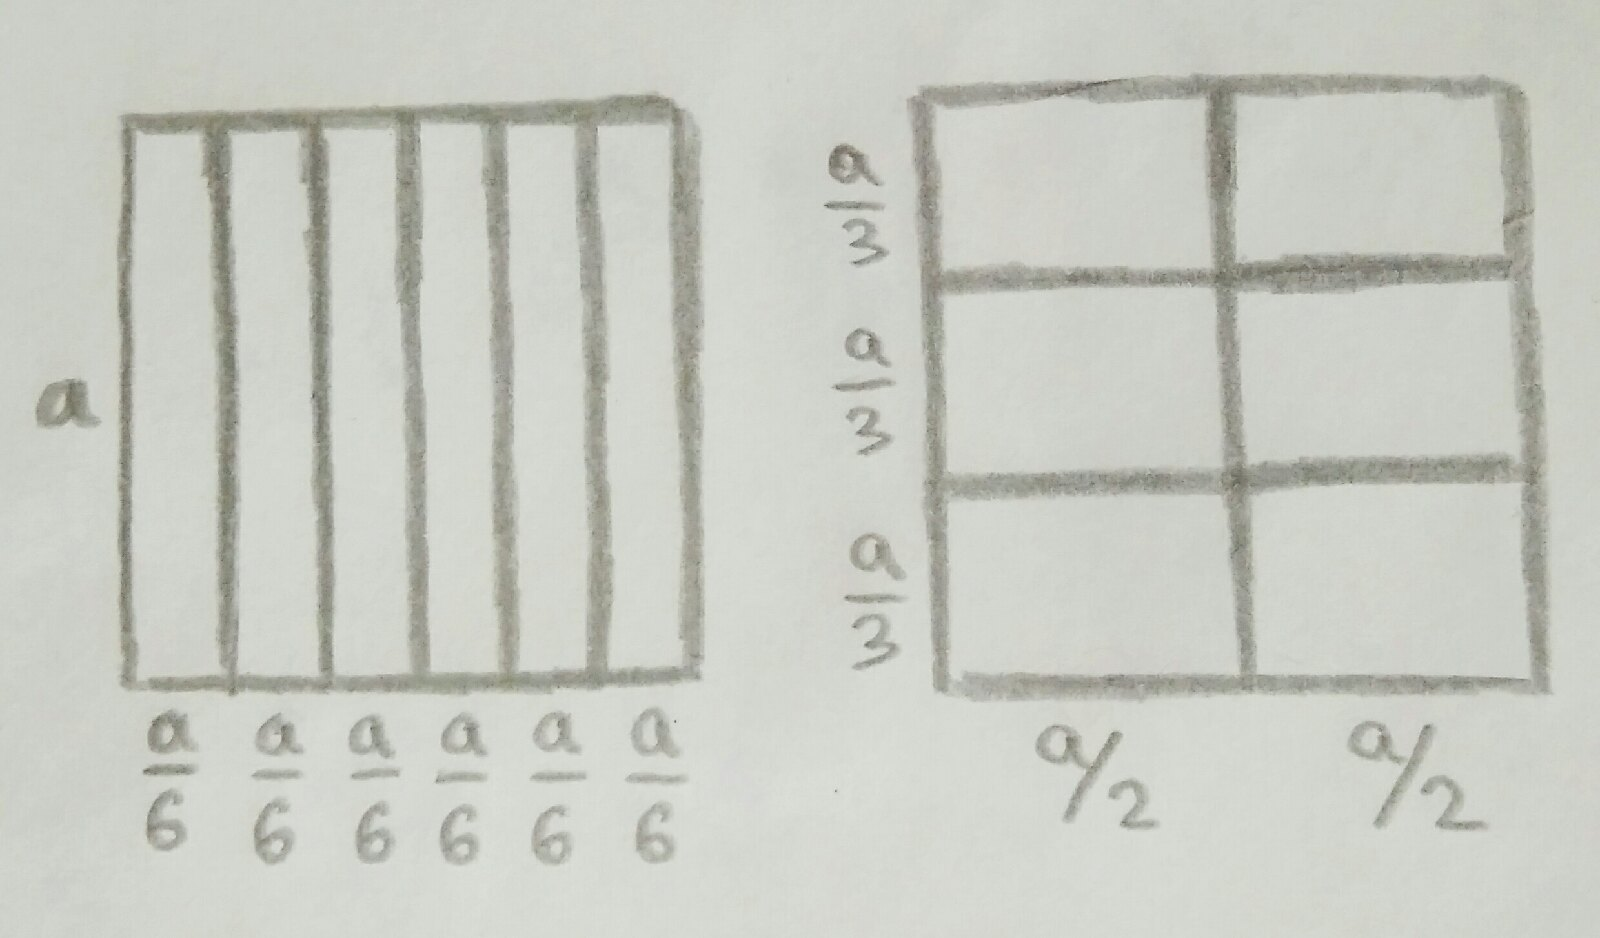
\includegraphics[width=\linewidth]{sol2.jpg}
        \end{figure}
    \end{minipage}
\end{minipage}

В первом случае периметр одной части будет равен $2\cdot(a + \frac16 a) = \frac73 a$.\\
Во втором же случае~--- $2\cdot(\frac12 a + \frac13 a) = 2\cdot\frac56a = \frac53 a$.\\
Если придумать ещё какой-нибудь способ разрезания (части же не обязаны быть прямоугольными) можно получить и другие ответы.\\ Поэтому здесь однозначного ответа НЕТ~--- задача не зафиксирована и ответ зависит от способа разрезания, а он нам не известен.
}
{Периметр квадрата до того, как его распилили, равен $4a$.\medskip\\
Площади всех получившихся частей одинаковы и равны $\frac16 a^2$.\medskip\\
Общая площадь четырёх частей равна $\frac23 a^2$.\medskip\\
Периметр зависит от способа разрезания.}{Подсказка}
\end{problem}

\begin{problem}{Умные вычисления.}{7.1.3}{6K}{(лёгкая)}
{Чему равно выражение $98 - 97 + 96 - 95 + \ldots - 3 + 2 - 1$?}
{НаписанноеРешение}
{ВерныйОтвет}{Подсказка}
\end{problem}

\begin{problem}{Умные вычисления.}{7.1.3}{6K}{(лёгкая)}
{Найти последнюю цифру числа $1 \cdot 2 + 2 \cdot 3 + 3 \cdot 4 + \ldots + 100 \cdot 101 + 101 \cdot 102$.}
{НаписанноеРешение}
{ВерныйОтвет}{Подсказка}
\end{problem}

\begin{problem}{Умные вычисления.}{7.1.3}{6K}{(лёгкая)}
{Найти суммы: $1 + 3 = {?}\qquad 1 + 3 + 5 = {?}\qquad 1 + 3 + 5 + 7 = {?}\qquad 1 + 3 + 5 + 7 + 9 = {?}$ \\Пользуясь этим, вычислить в уме сумму $1 + 3 + 5 + \ldots + 37 + 39 = {?}$}
{НаписанноеРешение}
{ВерныйОтвет}{Подсказка}
\end{problem}

\begin{problem}{Умные вычисления.}{7.1.3}{6K}{*}
{Железнодорожный билет для взрослого стоит $420$ рублей.\\ Стоимость билета для школьника составляет $40\%$ от стоимости билета для взрослого. Группа состоит из $15$ школьников и $4$ взрослых.\\ Вычисли в уме, сколько рублей стоят билеты на всю группу.}
{НаписанноеРешение}
{ВерныйОтвет}{Подсказка}
\end{problem}

\begin{problem}{Умные вычисления.}{7.1.3}{6K \textcolor{olive}{\textbf{$\spadesuit$}}}{(лёгкая)}
{\vspace{-6mm}\\\begin{minipage}{\linewidth}
    \begin{minipage}{0.5\linewidth}

    В квадрате, разделенном на четыре равные полоски, проведена диагональ. Чему равна площадь фигуры, закрашенной на рисунке, если сторона квадрата равна $1$ м?

    \end{minipage}
    \hspace{0.05\linewidth}
    \begin{minipage}{0.44\linewidth}
        \begin{figure}[H]
        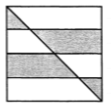
\includegraphics[width=\linewidth]{6K-17}
        \end{figure}
    \end{minipage}
\end{minipage}}
{НаписанноеРешение}
{ВерныйОтвет}{Подсказка}
\end{problem}

\begin{problem}{Умные вычисления.}{7.1.3}{6K \textcolor{olive}{\textbf{$\spadesuit$}}}{(лёгкая)}
{\vspace{-6mm}\\\begin{minipage}{\linewidth}
    \begin{minipage}{0.5\linewidth}

    Сколько треугольников изображено на рисунке?

    \end{minipage}
    \hspace{0.05\linewidth}
    \begin{minipage}{0.44\linewidth}
        \begin{figure}[H]
        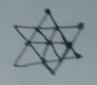
\includegraphics[width=\linewidth]{6K-33}
        \end{figure}
    \end{minipage}
\end{minipage}}
{НаписанноеРешение}
{ВерныйОтвет}{Подсказка}
\end{problem}

\begin{problem}{Умные вычисления.}{7.1.3}{6K \textcolor{olive}{\textbf{$\spadesuit$}}}{(лёгкая)}
{\vspace{-6mm}\\\begin{minipage}{\linewidth}
    \begin{minipage}{0.5\linewidth}

    На дорожках стадиона расставлены барьеры (их число на каждой дорожке указано на рисунке). Кенгуру хочет пробежать от старта до финиша, перепрыгивая через наименьшее число барьеров. Сколько раз кенгуру всё же придется прыгать через барьер?

    \end{minipage}
    \hspace{0.05\linewidth}
    \begin{minipage}{0.44\linewidth}
        \begin{figure}[H]
        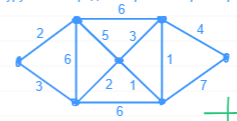
\includegraphics[width=\linewidth]{6K-25}
        \end{figure}
    \end{minipage}
\end{minipage}}
{НаписанноеРешение}
{ВерныйОтвет}{Подсказка}
\end{problem}

\begin{problem}{Умные вычисления.}{7.1.3}{6K \textcolor{olive}{\textbf{$\spadesuit$}}}{(лёгкая)}
{\vspace{-6mm}\\\begin{minipage}{\linewidth}
    \begin{minipage}{0.54\linewidth}

    Отрезок $AB$ несколько раз пересечен ломаной линией, как показано на рисунке справа.\smallskip\\ При этом получилось 5 квадратов.\medskip\\ Чему равна длина ломаной $AA_1A_2$\ldots$A_{10}B$, если известно, что длина $AB$ равна 10 см?

    \end{minipage}
    \hspace{0.05\linewidth}
    \begin{minipage}{0.4\linewidth}
        \begin{figure}[H]
        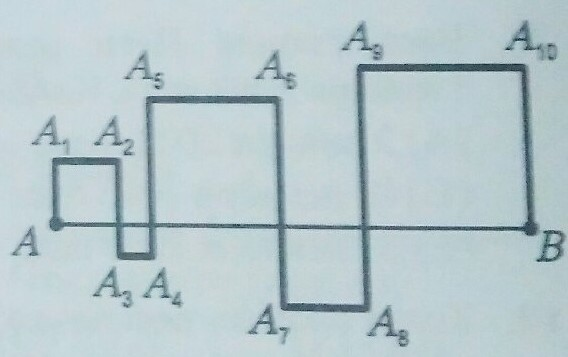
\includegraphics[width=\linewidth]{6K-38}
        \end{figure}
    \end{minipage}
\end{minipage}}
{НаписанноеРешение}
{ВерныйОтвет}{Подсказка}
\end{problem}

\begin{problem}{Умные вычисления.}{7.1.3}{6K \textcolor{olive}{\textbf{$\spadesuit$}}}{*}
{\vspace{-6mm}\\\begin{minipage}{\linewidth}
    \begin{minipage}{0.5\linewidth}

    Сколько на рисунке треугольников? \\(A) $6$; \\(B) $10$; \\(C) $12$; \\(D) $14$; \\(E) $16$.

    \end{minipage}
    \hspace{0.05\linewidth}
    \begin{minipage}{0.44\linewidth}
        \begin{figure}[H]
        
\includegraphics[width=\linewidth]{6K-24}
        \end{figure}
    \end{minipage}
\end{minipage}}
{НаписанноеРешение}
{ВерныйОтвет}{Подсказка}
\end{problem}

\begin{problem}{Математический язык.}{7.1.4}{6K}{*}
{На доске записан ряд из чисел и звёздочек: $5$, $*$, $*$, $*$, $*$, $*$, $*$, $8$.\\ Попробуй заменить звёздочки числами так, чтобы сумма каждых трёх чисел, стоящих подряд, равнялась $20$.}
{Попробуем перевести то, что мы имеем в данной задаче, на математический язык. Есть 6 чисел, обозначенных звёздочками, нам они пока не известны. Можно обозначить их неизвестными, например так: $\;5$, $a$, $b$, $c$, $d$, $e$, $f$, $8$.\\ Если сумма каждых трёх идущих подряд чисел равна 20, получаем шесть штук уравнений: $\,5 + a + b = 20$, \hfill $a + b + c = 20$, \hfill $b + c + d = 20$, \hfill $c + d + e = 20$, \hfill $d + e + f = 20$, \hfill $e + f + 8 = 20$. \\Даже несмотря на то, что такие задачи нам раньше не попадались, можно понять, что ничего страшного тут нет, ведь уравнений много. Проще всего использовать все уравнения по очереди, начиная с первого: \smallskip\\ $5 + a + b = 20 \;\Rightarrow\; a + b = 15 \;\Rightarrow\; 15 + c = 20 \;\Rightarrow\; c = 5 \;\Rightarrow\; d + e = 15 \;\Rightarrow\; f = 5$.\smallskip\\
А теперь в обратном порядке: $f = 5 \;\Rightarrow\; e + 5 + 8 = 20 \;\Rightarrow\; e = 7 \;\Rightarrow\; d = 20 - 7 - 5 = 8 \;\Rightarrow\; b + 5 + 8 = 20 \;\Rightarrow\; b = 7 \;\Rightarrow\; a = 20 - 5 - 7 = 8$.\\
Итого, у нас получилось найти все шесть неизвестных чисел.\\ Получается следующий ряд чисел: $\,5$, $8$, $7$, $5$, $8$, $7$, $5$, $8$.}
{$5$, $8$, $7$, $5$, $8$, $7$, $5$, $8$.\\
\textit{Комментарий:} других подходящих ответов у этой задачи нет. Отмечу, что вся задача так успешно решается, потому что {\slshape уравнений столько же, сколько и неизвестных}. Это то, что должно быть выполнено в любой стандартной задаче.}{Ввести шесть неизвестных и выписать все уравнения.\\ Главное при решении~--- внимательность и аккуратный порядок уравнений.}
\end{problem}

\begin{problem}{Математический язык.}{7.1.4}{6K \textcolor{red}{\textbf{$\spadesuit$}}}{(лёгкая)}
{Реши уравнение $\,x \cdot (x + 3{,}4) \cdot (1{,}4 - x) = 0$.\\ Выпиши все решения в порядке возрастания.}
{НаписанноеРешение}
{ВерныйОтвет}{Подсказка}
\end{problem}

\begin{problem}{Математический язык.}{7.1.4}{6K}{*}
{От города $A$ до города $B$ расстояние $40$ км. Два велосипедиста выехали из $A$ и $B$ одновременно навстречу друг другу, один со скоростью $15$ км/ч, а другой~--- $25$ км/ч. Вместе с первым из $A$ со скоростью $50$ км/ч вылетела безумная муха, долетела до второго, села ему на лоб, развернулась, полетела обратно к первому, села на лоб, вернулась ко второму, и так далее, пока велосипедисты не встретились, не столкнулись лбами и не раздавили муху. Сколько она пролетела километров?}
{НаписанноеРешение}
{ВерныйОтвет}{Подсказка}
\end{problem}

\begin{problem}{Математическая модель.}{7.1.5}{6K}{*}
{Творческая задача: некто сделал $1500$ шагов в одном направлении и оказался там же, где и был. Что произошло? Знаешь ли ты кого-то (например, персонажа из сказки), с кем такое могло случиться?}
{НаписанноеРешение}
{ВерныйОтвет}{Подсказка}
\end{problem}

\begin{problem}{Математическая модель.}{7.1.5}{6S}{(лёгкая)}
{Сколько было брёвен, если после 52 распилов получили 72 полена?}
{НаписанноеРешение}
{ВерныйОтвет}{Подсказка}
\end{problem}

\begin{problem}{Математическая модель.}{7.1.5}{6S}{(лёгкая)}
{По углам и сторонам квадрата вбиты колышки на расстоянии 2 м друг от друга.\\ Сколько колышков вбито, если сторона квадрата равна 10 м?}
{НаписанноеРешение}
{ВерныйОтвет}{Подсказка}
\end{problem}

\begin{problem}{Математическая модель.}{7.1.5}{6S}{(лёгкая)}
{Если на прямой через равные промежутки поставить 10 точек, то они займут отрезок длины $s$, если же поставить 100 точек, то отрезок длины $S$.\\ Во сколько раз $S$ больше $s$?}
{НаписанноеРешение}
{ВерныйОтвет}{Подсказка}
\end{problem}

\begin{problem}{Математическая модель.}{7.1.5}{6K}{(лёгкая)}
{На поверхности глобуса фломастером проведены 12 параллелей и 22 меридиана.\\ На сколько частей проведённые линии разделили поверхность глобуса?\smallskip\\
\textit{Меридиан}~--- это дуга окружности, соединяющая Северный и Южный полюсы.\\ \textit{Параллель}~--- это окружность, лежащая в плоскости, параллельной экватору.}
{НаписанноеРешение}
{ВерныйОтвет}{Подсказка}
\end{problem}

\begin{problem}{Математическая модель.}{7.1.5}{6S}{(лёгкая)}
{Как, имея два сосуда ёмкостью 5 л и 9 л, набрать из источника ровно 3 л воды?}
{НаписанноеРешение}
{ВерныйОтвет}{Подсказка}
\end{problem}

\begin{problem}{Математическая модель.}{7.1.5}{6K}{(лёгкая)}
{Три вора украли у чародея колбу с $24$ унциями волшебного зелья. Спешно унося ноги, они встретили в лесу продавца стеклянной посуды, у которого приобрели три сосуда. Найдя укромное местечко, воры решили разделить добычу, но тут обнаружили, что вместимость сосудов $5$, $11$ и $13$ унций.\\ Как им разделить между собой зелье поровну? Выливать зелье нельзя.}
{НаписанноеРешение}
{ВерныйОтвет}{Подсказка}
\end{problem}

\begin{problem}{Математическая модель.}{7.1.5}{6K}{*}
{В девятиэтажном доме один подъезд, на каждом этаже $4$ квартиры (в ряд).\\ Какому минимальному количеству жителей нужно выдать дрели, чтобы у каждого жителя в квартире было шумно? (либо есть дрель, либо через стену, пол или потолок есть <<шумный>> сосед с дрелью)}
{НаписанноеРешение}
{ВерныйОтвет}{Подсказка}
\end{problem}

\begin{problem}{Математическая модель.}{7.1.5}{6K \textcolor{red}{\textbf{$\spadesuit$}}}{(лёгкая)}
{В банку с водой влили стакан кислоты. Получился $10$-процентный раствор кислоты в воде. После этого в этот раствор добавили ещё два таких же стакана кислоты.\\ Кислота какой концентрации (в процентах) получилась в результате?}
{НаписанноеРешение}
{ВерныйОтвет}{Подсказка}
\end{problem}

\begin{problem}{Математическая модель.}{7.1.5}{6K}{(лёгкая)}
{На вопрос о возрасте его детей математик ответил: <<У нас с женой трое детей. Когда родился наш первенец, суммарный возраст членов семьи был равен $45$ годам, год назад, когда родился третий ребёнок~--- $70$ годам, а сейчас суммарный возраст детей~--- $14$ лет>>. Сколько лет каждому ребёнку, если известно, что у всех членов семьи дни рождения в один и тот же день?}
{Всего в задаче участвует 5 людей: математик, его жена, и три ребёнка. Обозначим возраст каждого буквой. Тогда получаем, что $a + b + 0 + 0 + 0 = 45$ (когда родился первенец, были только математик и его жена, а первенцу ещё не было и года). Год назад же картина была следующая: $(a\!+\!c) + (b\!+\!c) + c + d + 0 = 70$ (так как прошло столько лет, сколько первому ребёнку). После того как прошёл ещё год: $(c\!+\!1) + (d\!+\!1) + 1 = 14$.

Записываем систему уравнений: $\left\{\begin{aligned}
a + b = 45\\
a + b + 3c + d = 70\\
c + d + 3 = 14
\end{aligned}\right. \;\Rightarrow\; \left\{\begin{aligned}
3c + d &= 25\\
c + d &= 11
\end{aligned}\right.$

Вычитаем второе уравнение из первого, получаем, что $2c = 14 \;\Rightarrow\; c = 7$ и следовательно, $d = 11 - 7 = 4$. Это означает, что сейчас первенцу 8 лет, второму ребёнку --- 5 лет, а третьему --- 1 год.}
{Детям сейчас 8, 5 и 1 год, соответственно.}{Обозначь возраста всех участников задачи буквами. Сколько тогда лет прошло с рождения первенца до рождения третьего ребёнка?}
\end{problem}

\begin{problem}{Математическая модель.}{7.1.5}{6S}{(лёгкая)}
{Может ли в каком-то месяце быть 5 понедельников и 5 четвергов?}
{НаписанноеРешение}
{ВерныйОтвет}{Подсказка}
\end{problem}

\begin{problem}{Математическая модель.}{7.1.5}{6S}{(лёгкая)}
{В некотором месяце три пятницы были нечётными числами.\\ Какой день недели был 25-ого числа?}
{НаписанноеРешение}
{ВерныйОтвет}{Подсказка}
\end{problem}

\begin{problem}{Математическая модель.}{7.1.5}{6S}{(лёгкая)}
{Поезд имеет длину в 1 км и движется со скоростью 60 км/ч.\\ За какое время он пройдёт туннель длиной 1 км?}
{НаписанноеРешение}
{ВерныйОтвет}{Подсказка}
\end{problem}

\begin{problem}{Математическая модель.}{7.1.5}{6K}{(лёгкая)}
{Поезд из Москвы во Владивосток идёт $7$ дней и $1$ час. Каждый день в $12$ часов по московскому времени из этих городов выезжает по одному поезду.\\ Сколько поездов, вышедших из Владивостока, встретит поезд из Москвы?}
{НаписанноеРешение}
{ВерныйОтвет}{Подсказка}
\end{problem}

\begin{problem}{Математическая модель.}{7.1.5}{6K \textcolor{red}{\textbf{$\spadesuit$}}}{(лёгкая)}
{Есть рамка для фотографий со сторонами $22$ см и $60$ см (внешние размеры), толщина каёмки рамки~--- $1{,}5$ см.\\ Найти, во сколько раз внутренняя ширина рамки меньше внутренней длины.}
{НаписанноеРешение}
{ВерныйОтвет}{Подсказка}
\end{problem}

\begin{problem}{Математическая модель.}{7.1.5}{6K}{(лёгкая)}
{В прямоугольной комнате лежит большой ковёр, от которого до каждой стены ровно 25 сантиметров. Известно, что периметр ковра 25 метров.\\
Каковы в сумме длина и ширина комнаты?}
{Изобразим эту комнату: смотри рисунок ниже.\\
\begin{minipage}{\linewidth}
    \begin{minipage}{0.63\linewidth}
        Исходя из того, что периметр ковра 25 метров, нетрудно заключить, что сумма его длины и ширины вдвое меньше, то есть $a + b = 12{,}5$ метров. Теперь осталось как-то использовать расстояние до стен, равное 25 сантиметрам. Из рисунка видно, что тогда ширина комнаты на 50 сантиметров больше ширины ковра, и длина комнаты на 50 сантиметров больше длины ковра. Значит, сумма длины и ширины комнаты больше суммы длины и ширины ковра на метр и составляет $13{,}5$ метров.
    \end{minipage}
    \hspace{0.05\linewidth}
    \begin{minipage}{0.31\linewidth}
        \begin{figure}[H]
        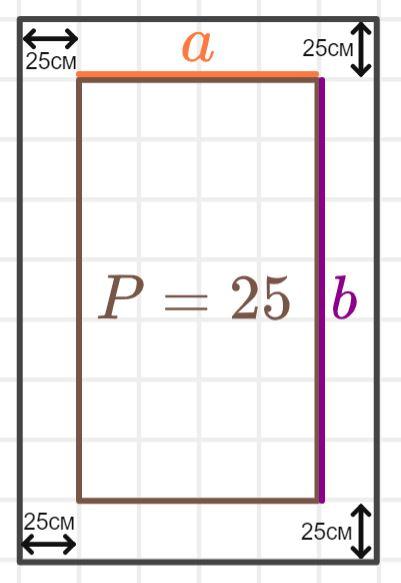
\includegraphics[width=\linewidth]{sol81}
        \end{figure}
    \end{minipage}
\end{minipage}}
{В сумме длина и ширина комнаты составляют $13{,}5$ метров.}{Для решения нужно нарисовать рисунок.}
\end{problem}

\begin{problem}{Математическая модель.}{7.1.5}{6K}{*}
{Михаил говорит, что выражение $w^{2} + 9$ всегда больше, чем $3w + 3w$.\\ Витя в ответ на это кричит: <<ты не прав, всё наоборот, $3w + 3w > w^{2} + 9$ всегда!>>\\ Петя, присоединяясь к разговору: Вы оба не правы!\\ Кто из них прав, и чем это можно обосновать? Что на самом деле верно?\smallskip\\ \hspace*{7cm}\fbox{$\vphantom{|}w^2 = w \cdot w$}}
{Нарисуем квадрат со стороной $w + 3$ и разделим его на 4 прямоугольника так, как показано на рисунке справа:\vspace{-10mm}\\\begin{minipage}{\linewidth}
    \begin{minipage}{0.56\linewidth}
    \vspace{10mm}
        Таким образом, Михаил и Витя спорят о том, сумма каких площадей больше~--- двух квадратов с площадями $w^2$ и $3^2 = 9$ соответственно или двух прямоугольников с площадью $3w$. Из рисунка кажется, что площадь квадратов должна быть больше.\\ Однако, понятно, что если взять $w = 3$, то $9 + 9 = 9 + 9$, все площади будут равны и получится равенство.\\ Так что Михаил и Витя неправы, а Петя прав.
    \end{minipage}
    \hspace{0.04\linewidth}
    \begin{minipage}{0.39\linewidth}
        \begin{figure}[H]
        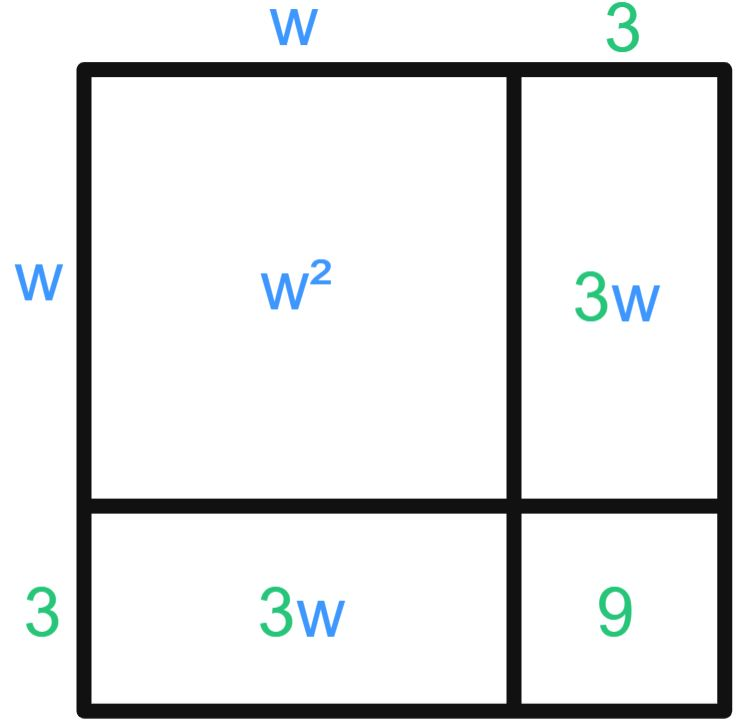
\includegraphics[width=\linewidth]{sol5}
        \end{figure}
    \end{minipage}
\end{minipage}
Строгое доказательство: мысленно представим похожий квадрат со стороной $w \!-\! 3$, его площадь (очевидно) будет не меньше 0, то есть $(w - 3)^2 \geqslant 0$.\\ Поскольку площадь суммы нескольких частей есть сумма площадей нескольких частей, $(w - 3)^2 = w^2 - 3w - 3w + 9$ (\textcolor{orange}{по факту это применение распределительного закона умножения}).\smallskip\\ Таким образом, $w^2 - 3w - 3w + 9 \geqslant 0$. Прибавляем к обеим частям $3w + 3w$:\\
$w^2 + 9 \geqslant 3w + 3w$. Это уже всегда верное утверждение (то есть Витя совсем не прав, а Михаил забыл, что возможно равенство при $w = 3$)}
{Прав Петя~--- Михаил забыл, что может быть равенство.\\ Доказательство использует свойства площади прямоугольников (3 класс) и \\распределительный закон.}{Надо нарисовать квадраты и прямоугольники со сторонами $w$ и $3$.}
\end{problem}

\begin{problem}{Математическая модель.}{7.1.5}{6K}{(лёгкая)}
{Всего есть $100$ кустов, Аня и Витя оба поливали кусты и каждый из них полил половину. $3$ самых красивых куста были политы и Аней, и Витей.\\ Сколько кустов остались не политыми?}
{НаписанноеРешение}
{ВерныйОтвет}{Подсказка}
\end{problem}

\begin{problem}{Математическая модель.}{7.1.5}{6K}{(лёгкая)}
{В Сеуле живёт $35$ покемонов.\\ Из них $22$ умеют приносить кофе, $13$ мастерски владеют расчёской. $10$ покемонов постоянно проливают кофе, а расчёску держат не той стороной.\\ Сколько Сеульских покемонов и умеют носить кофе, и владеют расчёской?}
{НаписанноеРешение}
{ВерныйОтвет}{Подсказка}
\end{problem}

\begin{problem}{Математическая модель.}{7.1.5}{6S}{(лёгкая)}
{Сестре втрое больше лет, чем было брату тогда, когда сестре было столько лет, сколько брату теперь.\\ Когда брату будет столько лет, сколько сестре сейчас, им вместе будет 28 лет.\\ Сколько сейчас лет сестре и сколько~--- брату?}
{НаписанноеРешение}
{ВерныйОтвет}{Подсказка}
\end{problem}

\begin{problem}{Математическая модель.}{7.1.5}{6K}{(лёгкая)}
{Сейчас мне вдвое больше лет, чем было ему тогда, когда мне было столько лет, сколько ему сейчас. Добавлю, что наш возраст вместе~--- $63$ года ровно.\\ Сколько сейчас лет каждому из нас?}
{НаписанноеРешение}
{ВерныйОтвет}{Подсказка}
\end{problem}

\begin{problem}{Математическая модель.}{7.1.5}{6K}{*}
{Три одинаковых прямоугольника склеили по сторонам так, что в итоге получился квадрат. Известно, что одна сторона прямоугольника равна $6$.\\ Найти площадь и периметр получившегося квадрата.}
{Есть только один способ, как получить квадрат~--- нужно склеить все три прямоугольника вместе по длинам. Это означает, что ширина прямоугольников втрое меньше, чем их длина (ведь иначе бы не получился квадрат).\smallskip\\
Нам известно, что одна сторона прямоугольника равна 6. Но какая? Ширина или длина? Это нам не известно, а значит, надо проверить оба варианта:\smallskip\\ Если длина равна 6, то ширина втрое меньше и равна 2.\smallskip\\ Если же ширина равна 6, то длина втрое больше и равна 18.\smallskip\\
Оба варианта изображены на рисунке ниже:\vspace{-3mm}\\\begin{minipage}{\linewidth}
    \hspace{0.02\linewidth}
    \begin{minipage}{0.42\linewidth}
        \begin{figure}[H]
        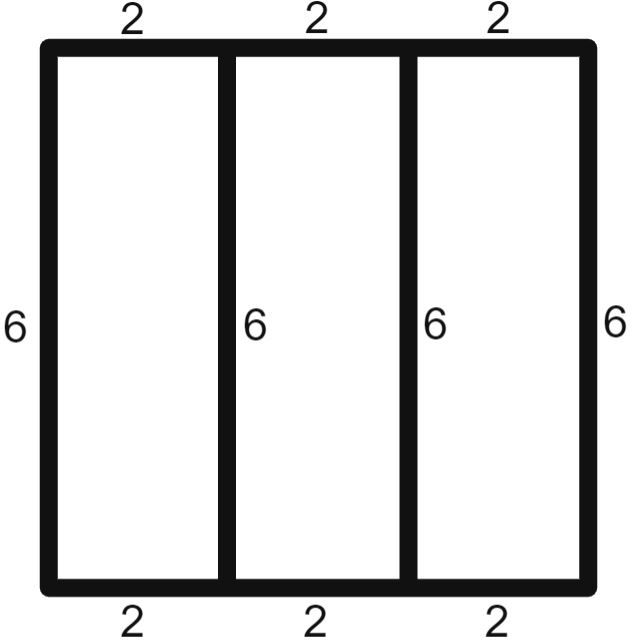
\includegraphics[width=\linewidth]{sol35}
        \end{figure}
    \end{minipage}
    \hspace{0.06\linewidth}
    \begin{minipage}{0.43\linewidth}
        \begin{figure}[H]
        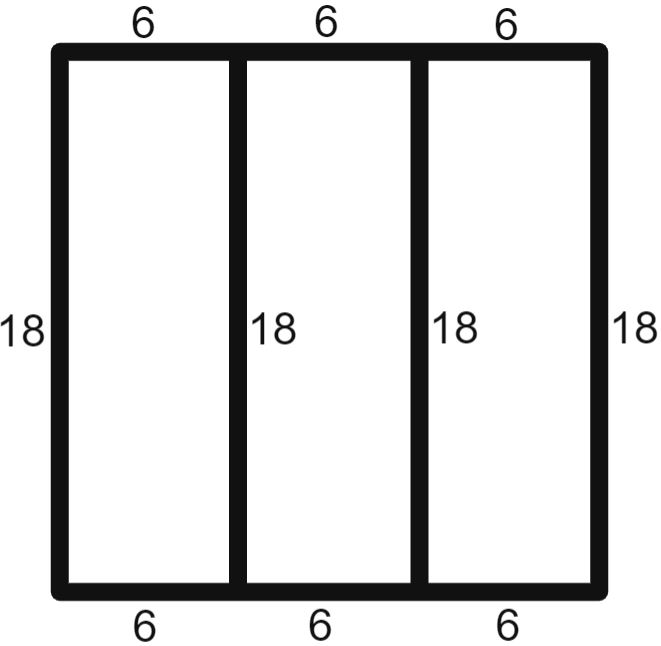
\includegraphics[width=\linewidth]{sol36}
        \end{figure}
    \end{minipage}
    \hspace{0.05\linewidth}
\end{minipage}
В первом случае сторона получившегося квадрата равна 6, поэтому периметр $P = 6 \cdot 4 = 24$, а площадь $S = 6 \cdot 6 = 36$.\smallskip\\
Во втором же случае сторона получившегося квадрата равна 18, поэтому периметр $P = 18 \cdot 4 = 72$, а площадь $S = 18 \cdot 18 = 324$.}
{Возможны два варианта: если длина прямоугольника равна 6, то $P = 24$ и $S = 36$. Если же ширина прямоугольника равна 6, то $P = 72$ и $S = 324$.}{Какая сторона прямоугольника равна 6? Это длина или ширина? Какой ответ получится в каждом случае?}
\end{problem}

\begin{problem}{Математическая модель.}{7.1.5}{6S}{*}
{Когда Коля был молод, как Оля, много лет было тётушке Поле~--- годом меньше, чем Коле теперь вместе с Олей.\\ Сколько лет было Коле, когда тётушка Поля была в возрасте Коли?}
{НаписанноеРешение}
{ВерныйОтвет}{Подсказка}
\end{problem}

\begin{problem}{Математическая модель.}{7.1.5}{6K}{*}
{Вычисли сумму чисел от $1$ до $n$.}
{НаписанноеРешение}
{ВерныйОтвет}{Нарисуй две <<лестницы>> из этих чисел.}
\end{problem}

\begin{problem}{Математическая модель.}{7.1.5}{6K red многопунктовая}{*}
{Найти сумму всех чисел методом <<лестницы>>:
\\a) $3$, $7$, $11$, $15$, $19$, $23$, $27$, $31$, $35$, $39$;
\\b) $1$, $3$, $5$, $7$, $9$, $\ldots$, $41$;
\\c) $-4$, $-1$, $2$, $5$, $8$, $\ldots$, $32$;
\\d) $a$, $a + 5$, $a + 10$, $\ldots$, $a + 5(n - 1)$, $a + 5n$.}
{НаписанноеРешение}
{ВерныйОтвет}{Подсказка}
\end{problem}

\begin{problem}{Математическая модель.}{7.1.5}{6K \textcolor{red}{\textbf{$\spadesuit$}} \textcolor{olive}{\textbf{$\spadesuit$}}}{*}
{\vspace{-6mm}\\\begin{minipage}{\linewidth}
    \begin{minipage}{0.5\linewidth}

    На куске шахматной доски (см. рисунок) расположены два белых и два чёрных коня. Ходы происходят по шахматным правилам. Могут ли через несколько ходов белые и чёрные кони поменяться местами?

    \end{minipage}
    \hspace{0.05\linewidth}
    \begin{minipage}{0.44\linewidth}
        \begin{figure}[H]
        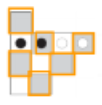
\includegraphics[width=\linewidth]{6K-20}
        \end{figure}
    \end{minipage}
\end{minipage}}
{НаписанноеРешение}
{ВерныйОтвет}{Подсказка}
\end{problem}

\begin{problem}{Составление выражений.}{7.1.6}{6S}{(лёгкая)}
{Если к задуманному числу прибавить 1, умножить сумму на 2, произведение разделить на 3 и отнять от результата 4, то получится 5.\\ Составить выражение, соответствующее этой ситуации.\\ Какое число было задумано?}
{Пусть задуманное число равно $x$.\\ Тогда $(x + 1)\cdot2 : 3 - 4 = 5$, это и есть выражение, соответствующее задаче.\\
1) Прибавим к обеим частям уравнения 4: $\; (x + 1)\cdot2 : 3 = 9$\\
2) Умножим обе части уравнения на 3: $\;\quad\;\:\; (x + 1)\cdot2 = 27$\\
3) Разделим обе части уравнения на 2: $\;\;\quad\quad\; x + 1 = 13{,}5$\\
4) Вычтем из обеих частей уравнения 1 и придём к ответу: $x = 12{,}5$.}
{Было задумано число $12{,}5$.}{Подсказка}
\end{problem}

\begin{problem}{Составление выражений.}{7.1.6}{6K}{(лёгкая)}
{На палке отмечены поперечные линии красного, жёлтого и зелёного цвета.\\ Если распилить палку по красным линиям, получится 15 кусков, если по жёлтым~--- 5 кусков, а если по зелёным~--- 7 кусков.\\ Сколько кусков получится, если распилить палку по линиям всех трёх цветов?}
{НаписанноеРешение}
{ВерныйОтвет}{Подсказка}
\end{problem}

\begin{problem}{Составление выражений.}{7.1.6}{6K \textcolor{olive}{\textbf{$\spadesuit$}}}{(лёгкая)}
{\vspace{-6mm}\\\begin{minipage}{\linewidth}
    \begin{minipage}{0.5\linewidth}

    Большой кубик склеен из маленьких деревянных кубиков. В нём просверлили $6$ сквозных дырок, параллельных ребрам (см. рисунок). Сколько маленьких кубиков остались неповрежденными?
    \\(A) $38$; \hfill (B) $40$; \hfill (C) $42$; \hfill (D) $44$; \hfill (E) $46$.

    \end{minipage}
    \hspace{0.05\linewidth}
    \begin{minipage}{0.44\linewidth}
        \begin{figure}[H]
        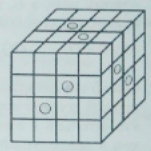
\includegraphics[width=\linewidth]{6K-28}
        \end{figure}
    \end{minipage}
\end{minipage}}
{НаписанноеРешение}
{ВерныйОтвет}{Подсказка}
\end{problem}

\begin{problem}{Составление выражений.}{7.1.6}{7A}{(лёгкая)}
{От двух шоколадок одинакового веса, но с различным процентным содержанием какао, отломили по куску равного веса. Каждый из отломанных кусков сплавили с остатком другого куска, после чего процентное содержание какао в обоих кусках стало одинаковым. Во сколько раз отломанный кусок меньше целой шоколадки?

}
{Предположим, что шоколадки имели вес $M$, а процентное содержание какао в них --- $r_1$ и $r_2$, соответственно. Допустим, что отломанный кусок имеет вес $m$. Тогда процентное содержание какао в первом куске составляет $$\frac{(M - m)\cdot\frac{r_1}{100} + m\cdot\frac{r_2}{100}}{M - m + m} = \frac{(M - m)\cdot r_1 + m\cdot r_2}{100M}$$
А во втором $$\frac{m\cdot\frac{r_1}{100} + (M - m)\cdot\frac{r_2}{100}}{m + M - m} = \frac{m\cdot r_1 + (M - m)\cdot r_2}{100M}$$
Так как нам известно, что эти выражения равны, приравниваем, и получаем, что $$\frac{(M - m)\cdot r_1 + m\cdot r_2}{100M} = \frac{m\cdot r_1 + (M - m)\cdot r_2}{100M} \;\Rightarrow\; (M \neq 0)$$ $$\Rightarrow\; (M - m)\cdot r_1 + m\cdot r_2 = m\cdot r_1 + (M - m)\cdot r_2 \;\Rightarrow\; (M - 2m)\cdot r_1 = (M - 2m)\cdot r_2$$
Следовательно, $(M - 2m)\cdot(r_1 - r_2) = 0$. Нам известно, что вначале процентное содержание какао в шоколадках разное, то есть $r_1 \neq r_2$ и $r_1 - r_2 \neq 0$.

Значит, $M - 2m = 0$. То есть $m = \frac12 M$, отломанный кусок меньше целой шоколадки вдвое.}
{Отломанный кусок меньше целой шоколадки вдвое --- шоколадку разломали пополам.}{Обозначь за $M$ вес всей шоколадки, за $m$ --- вес отломанного куска, за $r_i$ --- процент содержания какао в шоколадке №$i$.}
\end{problem}

\begin{problem}{Составление выражений.}{7.1.6}{6S}{(лёгкая)}
{Если в каждый подарочный пакет положить по 80 г пряников, то их останется 2 кг. Если же положить в каждый пакет по 100 г, то для заполнения всех пакетов не хватит 200 г. Сколько детей должны получить подарки?}
{Пусть подарочных пакетов было $n$, а общий вес пряников~--- $x$ грамм.\\ Нам надо найти $n$. Составим уравнения по задаче:\\
$x = 80\cdot n + 2000$ (2 кг = 2000 г) \\ $x = 100\cdot n - 200$ (раз не хватило 200 г, $x$ на 200 г меньше чем $100n$)\\
Получаем $80n + 2000 = 100n - 200 \;\Rightarrow\; 20n = 2200 \;\Rightarrow\; n = 110$.\\ Значит, подарочных пакетов было 110 (и детей, видимо, тоже)}
{Подарки должны получить 110 детей.}{Пусть пакетов было $n$, а общий вес пряников~--- $x$ грамм...}
\end{problem}

\begin{problem}{Составление выражений.}{7.1.6}{6K}{(лёгкая)}
{Лодка плывёт сначала полчаса по озеру, а потом полчаса по впадающей в это озеро реке. Написать выражение для длины $S$ общего пройденного лодкой маршрута, если скорость лодки равна $V$ км/ч, а скорость течения реки составляет $2$ км/ч.\\ Можем ли мы установить, с какой скоростью двигалась моторная лодка, если известно, что общее пройденное расстояние равно $31$ км?}
{Выражение (для чего бы то ни было) должно что-то выражать.\\ Чтобы мы могли что-то узнать про расстояние, нужно знать про скорость и время (так как $s = v \cdot t$). Когда лодка движется по озеру, её скорость равна $V$ км/ч, а когда она будет после этого двигаться по впадающей в озеро реке, её скорость будет равна $V - 2$ км/ч (поскольку течение будет ей мешать)\\
Так как и по озеру, и по реке лодка плывёт полчаса, получаем, что по озеру лодка проплывёт $s_{\text{озеро}} = V \cdot \frac{1}{2} = \frac12 V$ км, а по реке $s_{\text{река}} = (V - 2) \cdot \frac12 = \frac12 V - 1$ км. Значит, общее расстояние, пройденное лодкой, равно $s = s_{\text{озеро}} + s_{\text{река}} = \frac12 V + \frac12 V - 1 = $\\
$ = V - 1$ км. Таким образом, $s = V - 1$ км.\smallskip\\ Если общее пройденное расстояние равно 31 км, то $31 = V - 1$ (км).\\ Следовательно, $V = 32$ и скорость лодки будет равна 32 км/ч.}
{$s = V - 1$ километр.\\ Если известно, что $s = 31$ км, то скорость моторной лодки равна $32$ км/ч.}{Достаточно помнить, что $s = vt$. Буква $V$ останется в ответе.}
\end{problem}

\begin{problem}{Составление выражений.}{7.1.6}{6K}{(лёгкая)}
{У Красной Шапочки было $n$ пирожков. Когда она проезжает мост, хитрые лисы забирают половину пирожков, а затем возвращают ей один пирожок обратно. Выразить (не словами, а через $n$~--- словами грусть Красной Шапочки не передать) число пирожков после того, как\\
a) Шапочка проехала один мост; \hfill b) Шапочка проехала два моста.}
{a) После того, как Шапочка проезжает мост, вначале количество пирожков у неё уменьшается вдвое и становится равным $\frac{n}{2}$, а потом хитрые лисы возвращают ей один пирожок, и в итоге у Шапочки остаётся $\frac{n}{2} + 1$ пирожок.\\ Итого, число пирожков после одного моста будет равно $\frac{n}{2} + 1$.\smallskip\\
b) После этого моста Шапочке нужно проехать ещё один.\\ Вначале количество пирожков уменьшается вдвое: $(\frac{n}{2} + 1) : 2 = \frac{n}{4} + \frac12$.\\ Потом один пирожок прибавляется, итого получается $\frac{n}{4} + \frac12 + 1 = \frac{n}{4} + \frac32$ пирожков.

}
{После проезда первого моста у Шапочки останется $\frac{n}{2} + 1$ пирожок, а после второго моста~--- $\frac{n}{4} + \frac32$ пирожков.}{Ответ является выражением, зависящим от $n$.}
\end{problem}

\begin{problem}{Составление выражений.}{7.1.6}{6K}{*}
{Написать выражение для количества грибов, которые собрали вместе Белоснежка и $7$ гномов, если Белоснежка нашла $28$ грибов, самый низкий гном нашёл $m$ грибов, а также известно, что количество грибов у соседних гномов, если упорядочить их по возрастанию, будет отличаться на $2$.}
{Мы знаем, что Белоснежка нашла 28 грибов, а самый низкий гном~--- $m$ грибов. Следующий по высоте гном нашёл то ли $m + 2$, то ли $m - 2$ гриба.\\ Рассмотрим эти два случая отдельно:\smallskip\\
1 случай: <<Низкие гномы находят меньше грибов>>. Тогда гномы, если упорядочить их по возрастанию, собрали соответственно $m$, $m + 2$, $m + 4$, $m + 6$, $m + 8$, $m + 10$, $m + 12$, а всего $m + m + 2 + \ldots + m + 12 = 7m + 2 + 4 + 6 + 8 + 10 + 12 = 7m + 42$.\\ Не забываем ещё 28 грибов, собранные Белоснежкой, итого $7m + 42 + 28 = 7m + 70$.\smallskip\\
2 случай: <<Низкие гномы находят больше грибов>>. Опять же, упорядочиваем гномов по росту, получаем $m$, $m - 2$, $m - 4$, $m - 6$, $m - 8$, $m - 10$, $m - 12$, а всего $m + \ldots + m - 12 = 7m - 2 - 4 - 6 - 8 - 10 - 12 = 7m - 42$.\\
Добавляем собранное Белоснежкой: $7m - 42 + 28 = 7m - 14$.\smallskip\\
Получается, что вместе они собрали либо $7m + 70$ грибов (если высокие гномы находят на 2 гриба больше), либо $7m - 14$ грибов (если высокие гномы находят на 2 гриба меньше и $m \geqslant 12$).}
{Вместе Белоснежка и 7 гномов собрали то ли $7m + 70$, то ли $7m - 14$ грибов~--- в зависимости от того, кто лучше собирает грибы, высокие гномы или низкие.\medskip\\
\textbf{P.S.} В обоих случаях собранные грибы можно поделить поровну между гномами (выражение всегда делится на 7, и выходит либо $m + 10$, либо $m - 2$).\\ Можно подумать, почему это так (аккуратно выписать пару примеров и придумать единый способ перераспределения грибов, чтобы у всех было поровну).}{Напиши, сколько грибов будет у каждого гнома, и найди, сколько всего будет грибов. Осторожно~--- есть два случая.}
\end{problem}

\begin{problem}{Составление выражений.}{7.1.6}{6K}{*}
{За контрольную работу по истории каждый из $25$ школьников $5$ класса получил одну из трёх оценок: <<$3$>>, <<$4$>> или <<$5$>>.\\ На сколько больше было пятёрок, чем троек, если сумма всех оценок равна $106$?}
{НаписанноеРешение}
{ВерныйОтвет}{Подсказка}
\end{problem}

\begin{problem}{Составление выражений.}{7.1.6}{6S \textcolor{red}{\textbf{$\spadesuit$}} матеммодель}{(лёгкая)}
{Как отмерить 15 минут, имея под рукой только 7- и 11-минутные песочные часы?

}
{НаписанноеРешение}
{ВерныйОтвет}{Подсказка}
\end{problem}

\begin{problem}{Составление выражений.}{7.1.6}{6S \textcolor{red}{\textbf{$\spadesuit$}} матеммодель}{(лёгкая)}
{Как при помощи чашечных весов без гирь разделить 24 кг гвоздей на две части~--- 9 кг и 15 кг?}
{НаписанноеРешение}
{ВерныйОтвет}{Подсказка}
\end{problem}

\begin{problem}{Составление выражений.}{7.1.6}{6K}{(лёгкая) (для получения <<квадратных>> уравнений не всегда нужен квадратный дом)}
{За столом сидят люди. По кругу идёт кулёк с семечками. Первый человек взял $1$ семечко, второй~--- $2$, третий~--- $3$ и так далее: каждый следующий берёт на одно семечко больше, чем предыдущий.\\ Известно, что на втором круге было взято в сумме на $100$ семечек больше, чем на первом. Сколько человек сидело за столом?}
{Пусть всего за столом сидело $n$ человек. Схематично изобразим на рисунках сколько семечек было взято на первом кругу, а сколько --- на втором. \smallskip\\ \hspace*{3cm}(нарисуем отдельно первый круг и отдельно второй) \\\begin{minipage}{\linewidth}
    \begin{minipage}{0.44\linewidth}
        \begin{figure}[H]
        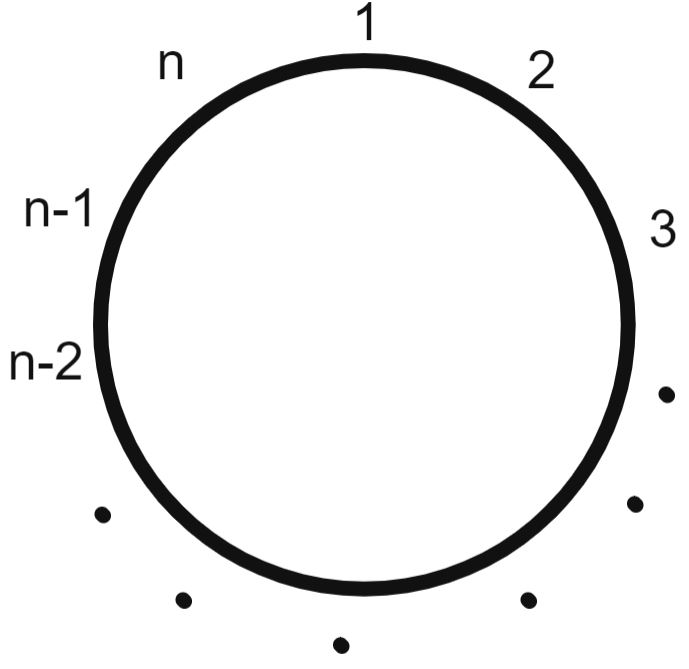
\includegraphics[width=\linewidth]{sol3}
        \end{figure}
    \end{minipage}
    \hspace{0.1\linewidth}
    \begin{minipage}{0.44\linewidth}
        \begin{figure}[H]
        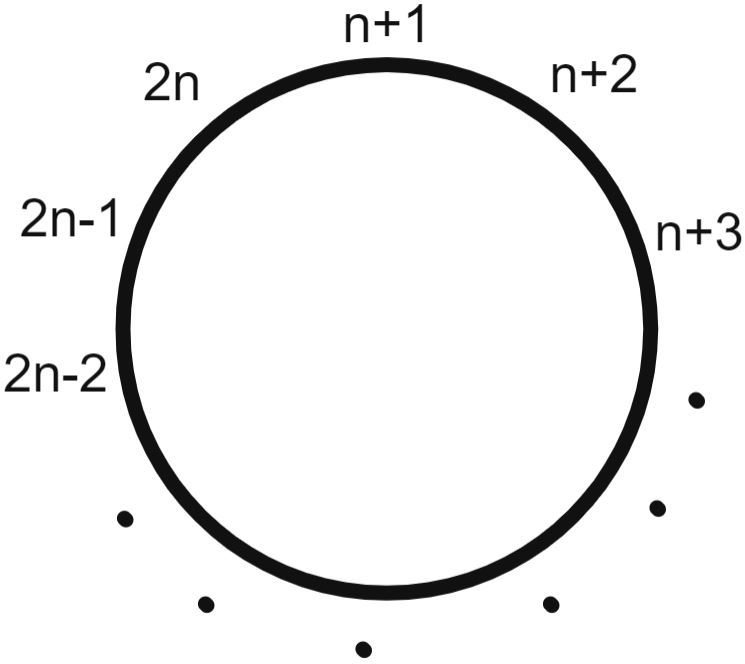
\includegraphics[width=\linewidth]{sol4}
        \end{figure}
    \end{minipage}
\end{minipage}
Как мы видим, на втором кругу \textbf{каждый} человек берёт ровно на $n$ семечек больше, чем он взял на первом кругу. Это логично, поскольку, чтобы вернуться к человеку, кулёк семечек должен пройти полный круг, а где бы не сидел человек, это значит, что количество семечек повысится на 1 ровно $n$ раз.\\ И поскольку каждый из $n$ человек взял на $n$ семечек больше на втором кругу, количество взятых семечек увеличилось на $n\cdot n = n^2$. Согласно задаче, это увеличение было равно 100 семечкам, отсюда получаем уравнение $n^2 = 100$.\\
Решение данного уравнения мы знаем из таблицы умножения, получаем $n = 10$ (отмечу, что $n = -10$ \textbf{тоже является решением}, но количество людей явно не может быть отрицательным). Таким образом, людей было 10.}
{За столом сидело 10 человек.}{На сколько больше семечек возьмёт каждый человек?\\ Какое уравнение тогда получается?}
\end{problem}

\begin{problem}{Составление выражений.}{7.1.6}{6K red квадратное, да ещё и с дробями}{*}
{Написать выражение для общего времени, которое автомобилист затратил на путь от Серпухова до квартиры в Москве, если от Серпухова до границы с Москвой автомобилист ехал $100$ километров по пробкам со скоростью $v$ км/ч, а после въезда в Москву его скорость возросла (так как в самой Москве пробок уже не было) на $40$ км/ч, и по Москве он проехал ещё $30$ километров.\\
Можем ли мы узнать начальную скорость автомобилиста, если общее время, которое он затратил на дорогу, равно: a) $5$ с половиной часов; b) $2$ часа $20$ минут?}
{Как мы знаем, если некоторое время $t$ ехать с одной и той же скоростью $v$, то пройденное расстояние $s = vt$. Поэтому $t = \frac{s}{v}$. Пока автомобилист едет до границы с Москвой, он проедет 100 километров за время $t_1 = \frac{100}{v}$ часов. По Москве он будет ехать с большей скоростью, а именно $v + 40$ км/ч, и затратит $t_2 = \frac{30}{v + 40}$ часов. Таким образом, общее время, которое автомобилист затратит на дорогу, равно $T = t_1 + t_2 = \frac{100}{v} + \frac{30}{v + 40}$ часов. Выражение успешно составлено!\smallskip\\
a) Получается уравнение $5{,}5 = \frac{100}{v} + \frac{30}{v + 40}$. Такие уравнения мы раньше не решали, можно угадать ответ подбором: при $v = 20$ км/ч получаем $\frac{100}{20} + \frac{30}{20 + 40} = 5 + \frac12 = 5{,}5$.\smallskip\\
b) Здесь получаем уравнение $2\frac13 = \frac{100}{v} + \frac{30}{v + 40}$, и после продолжительных попыток перебора в итоге получаем ответ $v = 50$ км/ч: $\frac{100}{50} + \frac{30}{50 + 40} = 2 + \frac13 = 2\frac13$.}
{a) $v = 20$ км/ч; $\;$ b) $v = 50$ км/ч.}{Чтобы составить выражение, используй формулу $s = vt$.\\ Полученные в итоге уравнения можно (и нужно) решить подбором.}
\end{problem}

\begin{problem}{Составление выражений.}{7.1.6}{6K}{*}
{Рядом стоят квадратный дом и дом, имеющий такую же ширину, как и первый, а длину~--- $7$ метров. Общая площадь первых этажей этих двух домов равна $60$ м$^{2}$.\\ Каковы размеры домов?\smallskip\\\textit{Указание:} Написать формулу для площади первого этажа квадратного дома, формулу для площади первого этажа второго дома, сложить, получить уравнение.\\ Подумать, умеем ли мы такое решать. Решить это уравнение методом подбора.}
{Поскольку нам неизвестна только сторона квадратного дома, обозначим её за $x$. Тогда площадь первого этажа квадратного дома будет равна $x \cdot x$. Второй дом имеет ширину $x$ метров и длину $7$ метров, площадь его первого этажа равна $7 \cdot x = 7x$. Получаем уравнение $x \cdot x + 7x = 60$.\\ С такими уравнениями мы ещё не встречались. Основная проблема в том, что есть $x \cdot x$~--- квадрат, а есть $7x$~--- прямоугольник, и сложить их и упростить выражение мы не можем (это почти как складывать яблоки с кирпичами).\\
Раз мы не умеем такое решать, просто угадаем ответ. $x = 1 \;\Rightarrow\; 1 + 7\cdot1 = 8 \neq 60$, $x = 2 \;\Rightarrow\; 2\cdot2 + 7\cdot2 = 18 \neq 60$, \hfill $x = 3 \;\Rightarrow\; 3\cdot3 + 7\cdot3 = 30 \neq 60$, $x = 4 \;\Rightarrow\; 4\cdot4 + 7\cdot4 = 44 \neq 60$,\hfill $x = 5 \;\Rightarrow\; 5\cdot5 + 7\cdot5 = 60 = 60$.\\ То есть ширина квадратного дома~--- 5 метров, и один дом имеет размеры $5\times5$ метров, а другой~--- $5\times7$ метров.}
{Дома имеют размеры $5\times5$ и $5\times7$ метров.}{Обозначь сторону квадратного дома за $x$.}
\end{problem}

\begin{problem}{Составление выражений.}{7.1.6}{6K \textcolor{olive}{\textbf{$\spadesuit$}}}{(лёгкая)}
{\vspace{-6mm}\\\begin{minipage}{\linewidth}
    \begin{minipage}{0.5\linewidth}

    На рисунке изображены 4 пересекающихся квадрата со сторонами 11, 9, 7, 5 см.\\
    На сколько $\text{см}^2$ сумма площадей двух серых областей больше суммы площадей двух красных областей?

    \end{minipage}
    \hspace{0.05\linewidth}
    \begin{minipage}{0.44\linewidth}
        \begin{figure}[H]
        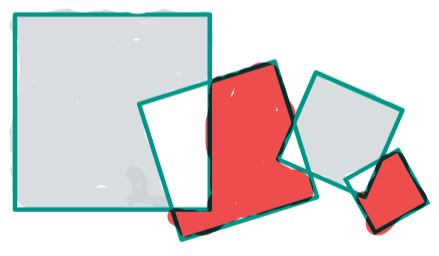
\includegraphics[width=\linewidth]{6K-39}
        \end{figure}
    \end{minipage}
\end{minipage}}
{НаписанноеРешение}
{ВерныйОтвет}{Подсказка}
\end{problem}

\begin{problem}{Составление выражений.}{7.1.6}{6K \textcolor{red}{\textbf{$\spadesuit$}} \textcolor{olive}{\textbf{$\spadesuit$}} алгебраические преобразования}{*}
{\vspace{-6mm}\\\begin{minipage}{\linewidth}
    \begin{minipage}{0.5\linewidth}

    На столе в виде треугольника выложены $28$ монет одинакового размера (см. рис.). Известно, что общая масса любой тройки монет, которые попарно касаются друг друга, равна $10$ г.\\ Найти суммарную массу всех $18$ монет на границе треугольника.

    \end{minipage}
    \hspace{0.05\linewidth}
    \begin{minipage}{0.44\linewidth}
        \begin{figure}[H]
        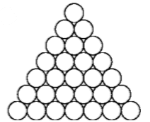
\includegraphics[width=\linewidth]{6K-2}
        \end{figure}
    \end{minipage}
\end{minipage}}
{НаписанноеРешение}
{ВерныйОтвет}{Подсказка}
\end{problem}

\begin{problem}{Составление выражений.}{7.1.6}{9I \textcolor{red}{\textbf{$\spadesuit$}} \textcolor{olive}{\textbf{$\spadesuit$}}}{*}
{\vspace{-9mm}\\\begin{minipage}{\linewidth}
    \begin{minipage}{0.5\linewidth}
    ~\vspace{2mm}\\
    Некто делает на заказ фенечку. Схема изображена  на рисунке справа: в первом и последнем ряду 4 узелка, во втором и третьем по 8, в четвёртом~--- 7, далее этот цикл повторяется (8 узелков в 5 и 6 рядах, 7 в седьмом, и так далее). В предпоследних двух рядах также по 8 узелков.
    \end{minipage}
    \hspace{0.05\linewidth}
    \begin{minipage}{0.44\linewidth}
        \begin{figure}[H]
        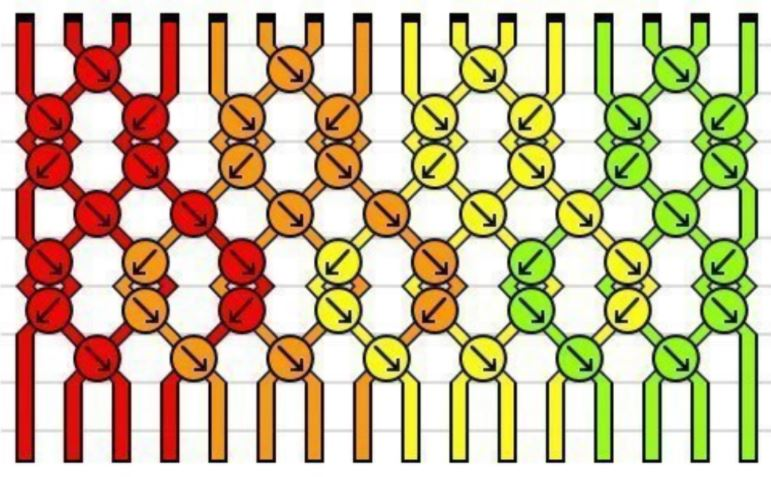
\includegraphics[width=\linewidth]{9I-1}
        \end{figure}
    \end{minipage}
\end{minipage}
Сколько сантиметров составит длина фенечки, если всего в ней 760 узелков, а пять рядов дают примерную длину в 1 см?}
{Условие означает, что количество узелков в рядах выглядит так: \\ $4{-}8{-}\textbf{8{-}7{-}8}{-}\ldots{-}\textbf{8{-}7{-}8}{-}8{-}4$. То есть повторяется шаблон с двумя рядами по 8 узелков и одним рядом с 7 узелками. Это означает, что всего в этом блоке из трёх рядов $8 + 8 + 7 = 23$ узелка. Как мы можем видеть, помимо этого повторяющегося блока ещё есть два ряда с 12 узелками вначале и два таких же ряда в конце.\\ Таким образом мы получаем уравнение на число узелков: если $k$ --- количество <<блоков>>, то $760 = 12 + 23\cdot k + 12$, откуда $736 = 23k \;\Rightarrow\; k = 736 : 23 = 32$.\\ Итого, есть два ряда вначале, потом 32 блока по три ряда каждый, потом два завершающих ряда. Значит, в фенечке всего $2 + 3\cdot32 + 2 = 4 + 96 = 100$ рядов. 5 рядов дают длину 1 см, а значит 100 рядов будут иметь длину $100 : 5 = 20$ см.}
{Длина этой фенечки составит примерно 20 сантиметров.}{Поскольку повторяется <<блок>> с двумя рядами по 8 узелков и одним рядом с 7 узелками, сперва посчитай, сколько всего узелков вне этих рядов, а затем составь выражение, если $k$ --- количество таких блоков.}
\end{problem}

\end{document}